\documentclass[a4paper,11pt]{article}
\usepackage{graphicx}
\usepackage{enumerate}
\usepackage[usenames, dvipsnames]{color}

\begin{document}

\begin{flushright}

\vspace{1.1cm}

{\bf\Huge Project 1}

\rule{0.25\linewidth}{0.5pt}

\vspace{0.5cm}
%Put Authors
Justin Ely
\linebreak
\newline
%Put Author's affiliations
\footnotesize{605.462 Data Visualization \\}
\vspace{0.5cm}
% Date here below
07 February, 2017
\end{flushright}

\noindent\rule{\linewidth}{1.0pt}

%%%%%%%%%%%%%%%%%%%%%%%%%%%%%%%%%%%%%%%%%%%%%%%%%%%%%%%%%%

\section{Pairing Wine and Food}

\begin{figure}[h!]
\caption{Program execution} 
\centering
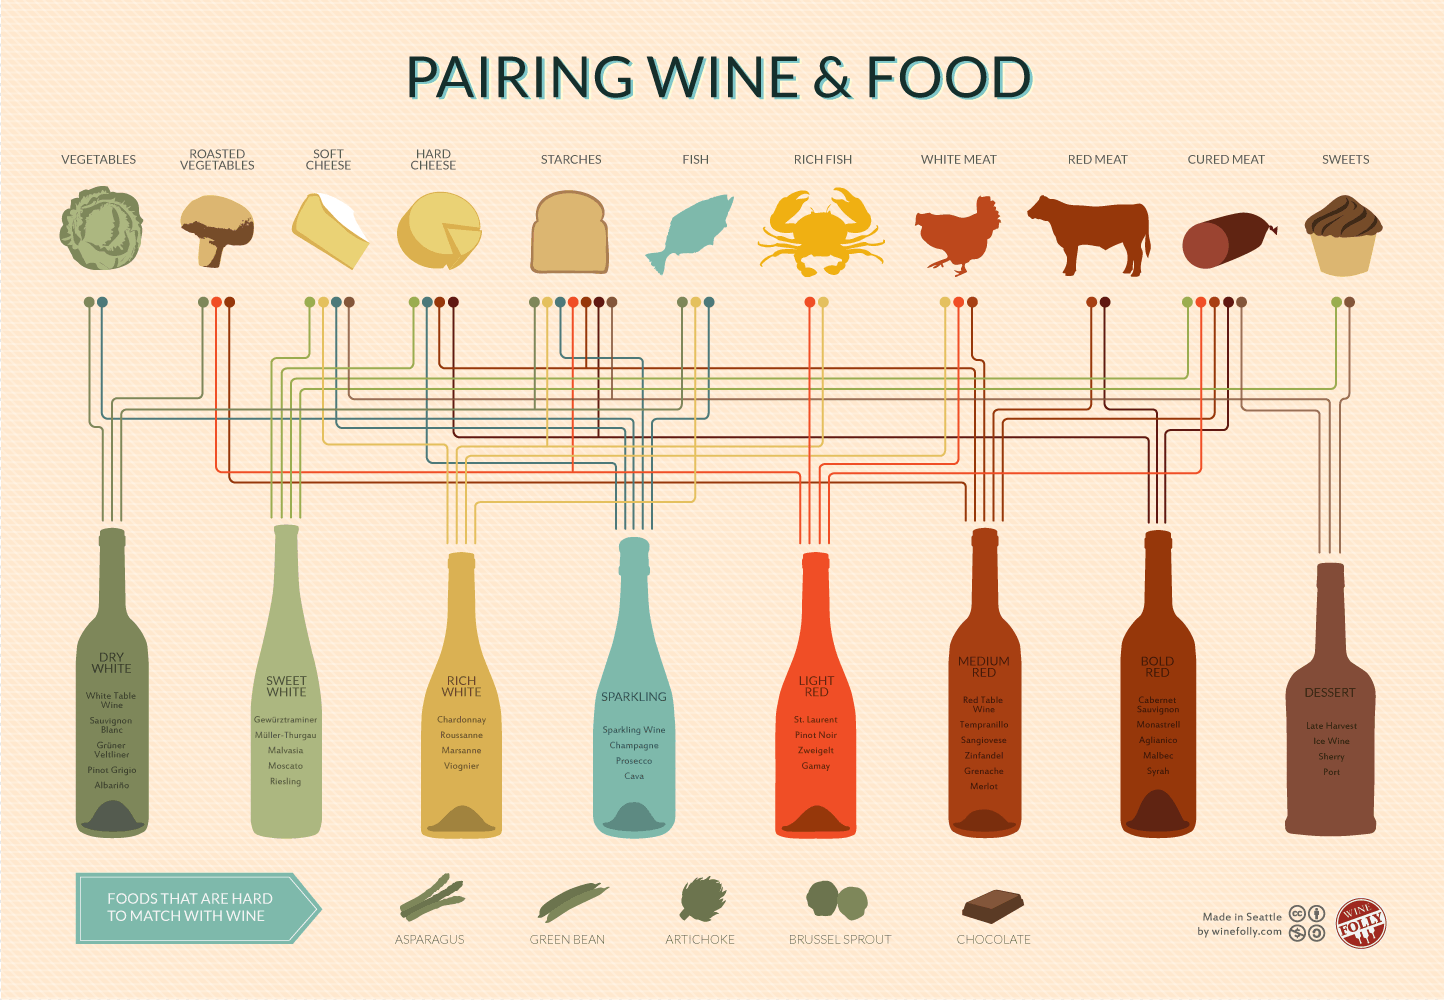
\includegraphics[width=1.1\textwidth]{wine-and-food-pairing-chart.png}
\end{figure}

\section{Type of Vizualization}

\section{Effective}
The pictorals of the food actually is an effective tool when this chart is used with just a quick glance.  Instead of having to read individual words, the eye can quickly jump to the meat, vegetables, etc very quickly.  

\section{Misleading}
The biggest bit of confusion is the mess of lines connecting the wine with the paired food options.  

The color-coding scheme of the wine bottles seems to {\it almost} make sense, but with just enough departures from a common scheme to adds to the ultimate confusion.  Light-red through dessert, each increasing in shade, makes sense with a mental perception of growing richness.  However, the other end of the spectrum makes little sense.  Sparkling wine is a blue color, and the progressing whites change from a golden to a deep green.  

One might think the colors map closely to the colors of the food on the top axis, but this doesn't hold up for many of the mappings.  For example, the sweet white (a pale green) doesn't map to a single vegetable.  The sparkling (blue) does map to the blue fish, but also maps to starches, both cheeses, and the vegetables.

The chart lines also seems to be in reverse oder.  The line terminated in a dot draws the eye from the bottom to the top, making the viewer use the chart in a wine to food direction.  This is opposite of typical usage, where someone would have a meal and need to find wine to pair with it.    

\section{Improvements}
The simplest and best improvement I could make to this mapping would be to make it interactive.  As someone selects either a bottle or a food, all others would fade into the background.  This would make the paths between the bottles stand out clearly, and avoid so much of the confusion in the middle.

Alternatively, if the chart must remain static, the wine bottles should be spread both above and below the food.  With the bottles more spread out, the criss-crossing lines will go down significantly and allow the paths to be more clearly traced.  

In either case, the colormaps need to be adjusted.  Since there's no consistent mapping between wine and food, this should be dropped and each axis should be allowed to take on a self-consistent progression.  Additionally, the colors need to be chosen to be more colorblind friendly.  Even to my very slight color-blindness, the pale greens and reds are difficult to distinguish when densely packed.  This would help not only making the graphic more accessible to the public, but also preserve the information in a B/W print.

%%%%%%%%%%%%%%%%%%%%%%%%%%%%%%%%%%%%%%%%%%%%%%%%%%%%%%%%%%


\end{document}
